前一节中,通过假设程序中的循环最终都会结束,编译器能够优化某些循环和包含这些循环的代码。优化器使用的基本逻辑是相同的:首先,假设程序不显示UB。然后,推导出必须为真的条件,使这个假设成立,并假设这些条件确实总是为真。最后,在这种假设下有效的优化都可以进行。如果违反了假设,优化器生成的代码会什么,我们无法知道(除了已经提到的限制,仍是在同一台计算机执行一些指令)。

标准中记录的每一个UB案例都可以转换为一个可优化的示例(特定的编译器是否能利用这一点就是另一回事了)。我们再看几个例子。

之前提到的,上溢有符号整数的结果是没有定义。编译器可以假设这种情况永远不会发生,并且使用正数对有符号整数进行递增,会得到一个更大的整数。编译器真的会执行这种优化吗?让我们来找找答案。比较\texttt{f()}和\texttt{g()}这两个函数:

\hspace*{\fill} \\ %插入空行
\noindent
\textbf{03\_int\_overflow.C}
\begin{lstlisting}[style=styleCXX]
bool f(int i) { return i + 1 > i; }
bool g(int i) { return true; }
\end{lstlisting}

定义良好的行为范围内,这些函数是相同的。可以对它们进行基准测试,以确定编译器是否会优化掉\texttt{f()}中的整个表达式。但如在前一章中看到的,有一种更可靠的方法。如果两个函数生成相同的汇编码,那么它们肯定是相同的。 

%\hspace*{\fill} \\ %插入空行
\begin{center}
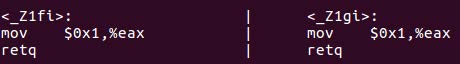
\includegraphics[width=0.7\textwidth]{content/3/chapter11/images/1.jpg}\\
图11.1 - GCC9生成的\texttt{f()}(左)和\texttt{g()}(右)函数的x86汇编输出
\end{center}

图11.1中,打开优化后,GCC确实为两个函数生成了相同的代码(Clang也是如此)。汇编中出现的函数的名称是所谓的“错误名称”:因为C++允许有不同参数列表的函数具有相同的名称,所以编译器必须为每个这样的函数生成一个唯一的名称,通过将所有参数的类型编码到对象代码中实际使用的名称中来进行实现。

如果想验证这段代码确实没有\texttt{?:}操作符的痕迹,最简单的方法是将\texttt{f()}函数与使用无符号整数进行相同计算的函数进行比较。参考以下代码:

\hspace*{\fill} \\ %插入空行
\noindent
\textbf{03\_int\_overflow.C}
\begin{lstlisting}[style=styleCXX]
bool f(int i) { return i + 1 > i; }
bool h(unsigned int i) { return i + 1 > i; }
\end{lstlisting}

无符号整数的溢出有良好的定义,\texttt{i + 1}是大于\texttt{i}不总是正确。

%\hspace*{\fill} \\ %插入空行
\begin{center}
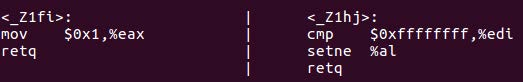
\includegraphics[width=0.9\textwidth]{content/3/chapter11/images/2.jpg}\\
图11.2 - GCC9生成的\texttt{f()}(左)和\texttt{h()}(右)函数的x86汇编输出
\end{center}

\texttt{h()}函数产生不同的代码,cmp指令会进行比较,不熟悉x86汇编也可以猜到。在左边,\texttt{f()}将载入常量0x1(布尔值也称为true),并将结果放在寄存器EAX中用于返回。 

这个例子还演示了试图推理UB或将其视为实现定义的危险。若程序将对整数做某种加法,当它溢出,特定的硬件将执行相应的操作,那么将得到错误的结果。编译器(有些编译器确实如此)生成的代码可能根本不需要递增指令。

现在,有了足够的知识来充分说明第2章中埋下的问题。在那一章中,我们观察到同一个函数的两个几乎相同的实现之间的性能差异。该函数的工作是一个字符一个字符地比较两个字符串,如果第一个字符串的字典序比第一个字符串大,则返回true。这是最简实现:

\hspace*{\fill} \\ %插入空行
\noindent
\textbf{04a\_compare1.C}
\begin{lstlisting}[style=styleCXX]
bool compare1(const char* s1, const char* s2) {
	if (s1 == s2) return false;
	for (unsigned int i1 = 0, i2 = 0;; ++i1, ++i2) {
		if (s1[i1] != s2[i2]) return s1[i1] > s2[i2];
	}
}
\end{lstlisting}

这个函数用于对字符串进行排序,因此基准测试测量了对特定输入字符串集进行排序的时间:

%\hspace*{\fill} \\ %插入空行
\begin{center}
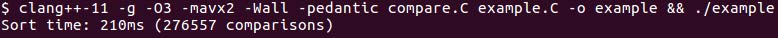
\includegraphics[width=0.9\textwidth]{content/3/chapter11/images/3.jpg}\\
图11.3 -使用\texttt{compare1()}函数进行字符串比较的排序基准测试
\end{center}

比较实现非常简单,这段代码中没有什么不必要的东西。然而,令人惊讶的结果是,这是代码性能最差的版本之一。表现最好的版本几乎是一样的:

\hspace*{\fill} \\ %插入空行
\noindent
\textbf{04b\_compare2.C}
\begin{lstlisting}[style=styleCXX]
bool compare2(const char* s1, const char* s2) {
	if (s1 == s2) return false;
	for (int i1 = 0, i2 = 0;; ++i1, ++i2) {
		if (s1[i1] != s2[i2]) return s1[i1] > s2[i2];
	}
}
\end{lstlisting}

唯一的区别是循环变量的类型:\texttt{unsigned int (compare1())}和\texttt{int (compare2())}。但索引不是负的,这应该没有任何区别,但实际的性能差异很大:

%\hspace*{\fill} \\ %插入空行
\begin{center}
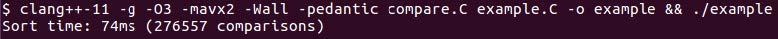
\includegraphics[width=0.9\textwidth]{content/3/chapter11/images/4.jpg}\\
图11.4 - 使用\texttt{compare2()}函数进行字符串比较的排序基准测试
\end{center}

这种显著的性能差异的原因与UB有关。为了理解发生了什么,必须再次检查汇编码。图11.5显示了GCC为这两个函数生成的代码(只显示了最相关的部分,字符串比较循环):

%\hspace*{\fill} \\ %插入空行
\begin{center}
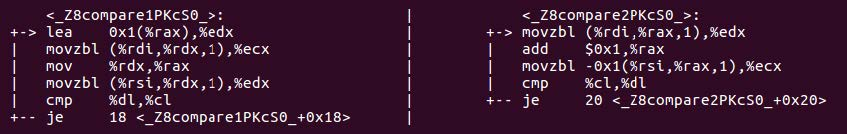
\includegraphics[width=0.9\textwidth]{content/3/chapter11/images/5.jpg}\\
图11.5 - 为\texttt{compare1()}(左)和\texttt{compare2()}(右)函数生成的x86汇编码
\end{center}

代码看起来非常相似,只有一个不同。在右边(\texttt{compare2()})中,可以看到add指令,它用于将循环索引加1(编译器通过用一个循环变量替换两个循环变量来优化代码)。在左边,没有看起来像加法或增量的指令。取而代之的是lea指令,它表示加载和扩展地址,这里用这种方式将索引变量增加1(进行了同样的优化,只有一个循环变量)。 

现在,应该能够猜到为什么编译器必须生成不同的代码。虽然开发者期望索引永远不会溢出,但是编译器不能做这样的假设。注意,两个版本都使用32位整数,但是代码是为64位机器生成的。如果一个32位的带符号int溢出,结果是未定义的,所以在这种情况下,编译器会假设溢出永远不会发生。如果操作没有溢出,则加法指令产生正确的结果。对于\texttt{unsigned int},编译器必须考虑溢出的可能性,递增\texttt{UINT\_MAX}应该得到0。但事实证明,x86-64上的add指令没有这些语义。相反,它将结果扩展为一个64位整数。x86上32位无符号整数算法的最佳选择是lea指令,它可以完成这项工作,但速度要慢得多。

这个示例演示了如何从程序定义良好且UB从未发生的假设往回推,编译器可以启用非常有效的优化,最终使整个排序操作快几倍。

既然已经理解了代码中发生的事情,就可以解释代码的其他几个版本的行为了。首先,使用64位整数,有符号的或无符号的,提供与32位有符号整数相同的性能,编译器将使用add(对于64位的无符号值,确实有正确的溢出语义)。其次,如果使用了最大索引,或者字符串长度,编译器将推断出索引不会溢出:

\begin{lstlisting}[style=styleCXX]
bool compare1(const char* s1, const char* s2,
unsigned int len) {
	if (s1 == s2) return false;
	for (unsigned int i1 = 0, i2 = 0; i1 < len; ++i1, ++i2) {
		if (s1[i1] != s2[i2]) return s1[i1] > s2[i2];
	}
	return false;
}
\end{lstlisting}

不必要的长度比较使得这个版本比最好的版本稍微慢一些。要避免意外地遇到这个问题,最可靠的方法是始终使用有符号循环变量或硬件本地大小的无符号整数(因此,除非真的需要,否则避免在64位处理器上执行无符号整型运算)。

可以使用标准中描述为未定义行为的其他情况,构造类似的演示(尽管不能保证特定的编译器会利用可能的优化)。下面是使用指针解引用的例子:

\hspace*{\fill} \\ %插入空行
\noindent
\textbf{06a\_null.C}
\begin{lstlisting}[style=styleCXX]
int f(int* p) {
	++(*p);
	return p ? *p : 0; // Optimized to: return *p
}
\end{lstlisting}

这是一种常见的情况的简化,开发者编写了指针检查代码,以防止空指针,但并没有在所有地方这样做。如果输入参数是空指针,则第二行(增量)是UB,这意味着整个程序的行为未定义,因此编译器可以假设它从未发生。对汇编代码的检查表明,第三行中的比较被消除了:

%\hspace*{\fill} \\ %插入空行
\begin{center}
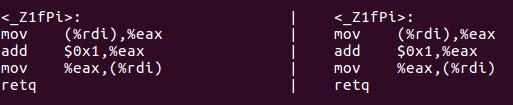
\includegraphics[width=0.9\textwidth]{content/3/chapter11/images/6.jpg}\\
图11.6 -带(左)和不带(右)操作符的\texttt{f()}函数生成的x86汇编码
\end{center}

如果先做指针检查,也会发生同样的情况:

\hspace*{\fill} \\ %插入空行
\noindent
\textbf{07a\_null.C}
\begin{lstlisting}[style=styleCXX]
int f(int* p) {
	if (p) ++(*p);
	return *p;
}
\end{lstlisting}

同样,对汇编代码的检查表明,指针比较已经消除了,尽管到目前为止的程序行为都定义得很好。如果指针\texttt{p}不为空,则比较是多余的,可以省略。如果\texttt{p}为空,程序的行为是未定义的,这意味着编译器可以做任何它想做的事情。这里,它想做的是忽略比较。最终结果是,无论\texttt{p}是否为空,都可以消除比较。

上一章中,我们花了大量的时间来分析哪些优化是可能的,因为编译器可以证明它们是安全的。这里,将重新讨论这个问题。首先,这对于理解编译器优化绝对有必要。其次,这与UB有关系。当编译器从一个特定的语句中推断出一些信息时(比如从\texttt{return}语句推断出的\texttt{p}是非空的),这些信息不仅可以用于优化后面的代码,还可以用于优化前面的代码。传播这些信息的限制来自于编译器可以确定的其他信息。为了演示,稍微修改一下前面的例子:

\hspace*{\fill} \\ %插入空行
\noindent
\textbf{08a\_null.C}
\begin{lstlisting}[style=styleCXX]
extern void g();
int f(int* p) {
	if (p) g();
	return *p;
}
\end{lstlisting}

这种情况下,编译器不会消除指针检查,这可以在生成的汇编代码中看到:

%\hspace*{\fill} \\ %插入空行
\begin{center}
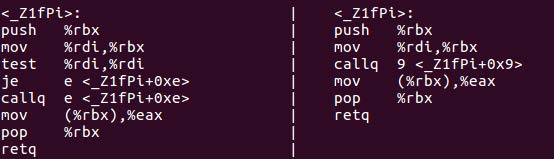
\includegraphics[width=0.9\textwidth]{content/3/chapter11/images/7.jpg}\\
图11.7 - 为\texttt{f()}函数生成的x86汇编码(左)和(右)没有指针检查
\end{center}

测试指令执行与null(零)的比较,后面跟着条件跳转——这就是\texttt{if}语句在汇编中的样子。 

为什么编译器没有优化掉检查呢?要回答这个问题,必须弄清楚在什么条件下优化会改变程序的(良好定义的)行为。

要使优化无效,需要以下两点:

\begin{itemize}
\item 
首先,\texttt{g()}函数必须知道指针\texttt{p}是否为空。这是可能的,例如:\texttt{p}也可以让\texttt{f()}的调用者存储在一个全局变量中。

\item 
其次,如果\texttt{p}为空,则不能执行\texttt{return}。这也是可能的:如果\texttt{p}为空,\texttt{g()}可能会抛出一个异常。
\end{itemize}

对于与UB密切相关的C++优化的最后一个例子,将看一些不同的东西。\texttt{const}关键字对优化的影响,这将说明为什么编译器不能成功的优化某些代码。

\begin{lstlisting}[style=styleCXX]
bool f(int x) { return x + 1 > x; }
\end{lstlisting}

正如所看到的,优化编译器将从这个函数中删除所有代码,并将其替换为\texttt{return true}。现在让函数做更多的工作:

\begin{lstlisting}[style=styleCXX]
void g(int y);
bool f(int x) {
	int y = x + 1;
	g(y);
	return y > x;
}
\end{lstlisting}

当然,可能会有同样的优化,代码可以重写如下:

\begin{lstlisting}[style=styleCXX]
void g(int y);
bool f(int x) {
	g(x + 1);
	return x + 1 > x;
}
\end{lstlisting}

必须调用\texttt{g()},但函数仍然返回true。在不陷入未定义行为的情况下,比较不会产生结果。同样,大多数编译器都会进行这种优化。以通过比较原始代码生成的汇编码,和完全手工优化的代码生成的汇编码来证实这一点:

\begin{lstlisting}[style=styleCXX]
void g(int y);
bool f(int x) {
	g(x + 1);
	return true;
}
\end{lstlisting}

可能进行优化的原因是\texttt{g()}函数不更改其参数。同一段代码中,如果\texttt{g()}通过引用接收实参,则不再可能进行优化:

\begin{lstlisting}[style=styleCXX]
void g(int& y);
bool f(int x) {
	int y = x + 1;
	g(y);
	return y > x;
}
\end{lstlisting}

现在\texttt{g()}函数可以改变\texttt{y}的值,所以每次都要进行比较。如果函数\texttt{g()}的目的不是改变它的参数,就可以通过值进行传递。另一个选项是传递\texttt{const}引用,虽然对于小型类型(如整数)没有理由这样做,但模板代码通常会生成这样的函数。这个例子中,代码看起来会是这样:

\hspace*{\fill} \\ %插入空行
\noindent
\textbf{10\_const.C}
\begin{lstlisting}[style=styleCXX]
void g(const int& y);
bool f(int x) {
	int y = x + 1;
	g(y);
	return y > x;
}
\end{lstlisting}

对汇编程序的检查表明\texttt{return}语句没有进行优化,仍然进行比较。当然,编译器不做某种优化证明了什么,说明没有优化器是完美的,但不做优化是有原因的。不管代码怎么样,C++标准并不保证\texttt{g()}函数不改变它的参数!下面是一个完全符合标准的实现:

\begin{lstlisting}[style=styleCXX]
void g(const int& y) { ++const_cast<int&>(y); }
bool f(int x) {
	int y = x + 1;
	g(y);
	return y > x;
}
\end{lstlisting}

函数允许弃用\texttt{const}。结果定义的很好,并在标准中指定(这并不能使它成为好的代码,只是有效的代码)。但是,有一个例外:在创建时声明为\texttt{const}的对象转换为\texttt{const}。举例来说,这是一个很好的定义(但不明智):

\begin{lstlisting}[style=styleCXX]
int x = 0;
const int& y = x;
const_cast<int&>(y) = 1;
\end{lstlisting}

这是会有UB的版本:

\begin{lstlisting}[style=styleCXX]
const int x = 0;
const int& y = x;
const_cast<int&>(y) = 1;
\end{lstlisting}

可以通过将中间变量\texttt{y}声明为\texttt{const}来利用UB:

\begin{lstlisting}[style=styleCXX]
void g(const int& y);
bool f(int x) {
	const int y = x + 1;
	g(y);
	return y > x;
}
\end{lstlisting}

现在编译器可以假设函数总是返回true。更改它的唯一方法是创造UB,而编译器不需要UB。在写这本书的时候,还不知道有编译器会做这种优化。

考虑到这一点,在对使用\texttt{const}来进行优化,有什么建议呢?

\begin{itemize}
\item 
如果值没有改变,将它声明为\texttt{const}。正确性很重要,但这确实可以支持一些优化,特别是当编译器可以通过在编译时计算表达式来传播\texttt{const}时。

\item 
更好的优化方法是,若该值在编译时已知,则将其声明为\texttt{constexpr}。

\item 
通过\texttt{const}引用传递形参给函数没有任何优化作用,因为编译器必须假定函数可能会抛弃\texttt{const}(如果函数是内联的,编译器知道发生了什么,但如何声明形参就无关紧要了)。另一方面,这是将\texttt{const}对象传递给函数的唯一方法,因此,只要有可能,请将引用声明为\texttt{const}(更重要的为了清晰的表明意图)。

\item 
对于小类型,按值传递比按引用传递更有效(这不适用于内联函数)。这很难与模板生成的泛型函数相协调(不要假设模板总是内联的,大型模板函数通常不是)。有一些方法可以强制特定类型的值传递,但会使模板代码更加繁琐。不要一开始就写这样的代码,只有当测试结果表明,对于特定的代码段,这种工作是合理的时再这样做。

\end{itemize}

我们已经详细探讨了C++中的UB如何影响C++代码的优化。现在是时候回到正题,了解如何在自己的程序中利用UB了。
























